\hsection{Python under Ubuntu Linux}%
%
\begin{figure}%
\centering%
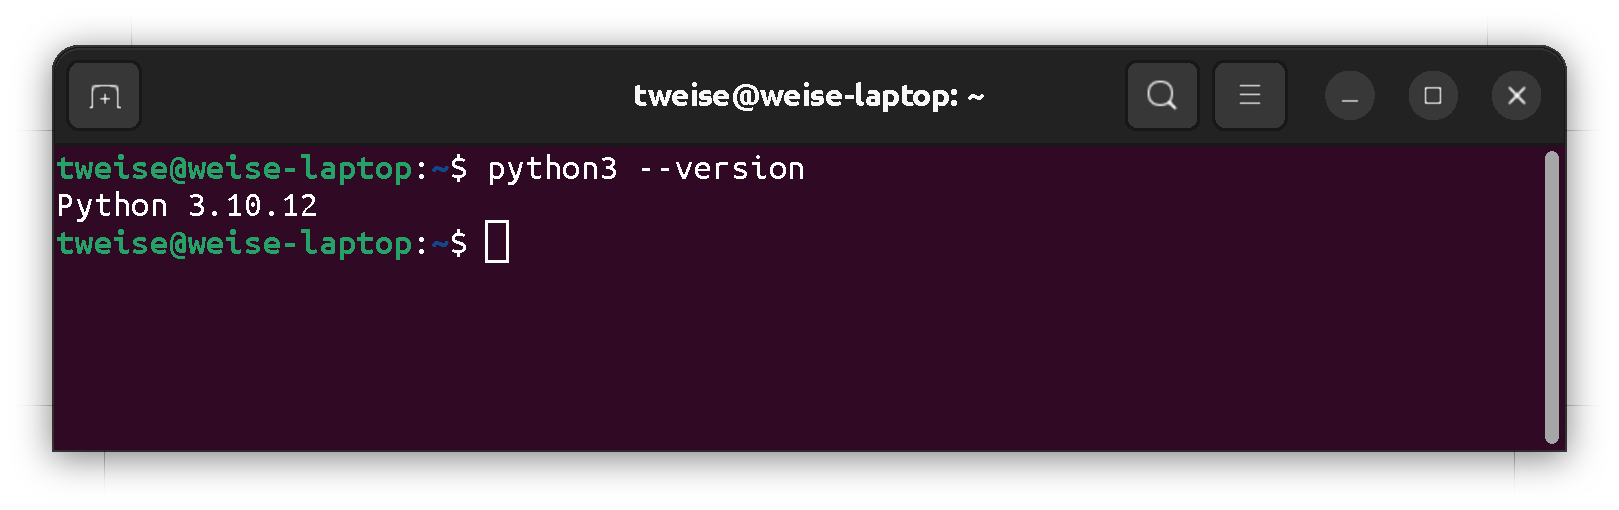
\includegraphics[width=0.7\linewidth]{\currentDir/ubuntuTerminalPythonVersion}%
\caption{Under my \ubuntu\ \linux~\softwareStyle{22.04} system, typing \bashil{python3 --version} in a \pgls{terminal} and hitting return yields version~\softwareStyle{3.10.12}.}%
\label{fig:ubuntuTerminalPythonVersion}%
\end{figure}%
%
\begin{sloppypar}%
Under \ubuntu\ \linux, \python~\softwareStyle{3} is already pre-installed.
You can open a \pgls{terminal}~\cite{B2022ELATCL} by pressing~\ubuntuTerminal, then type in \bashil{python3 --version}, hit \keys{\enter}, and get the result illustrated in \cref{fig:ubuntuTerminalPythonVersion}:
\end{sloppypar}%
%
\FloatBarrier%
\endhsection%
%
